\subsection{Data Access Layer}


\subsection{Data Access Layer}


\subsection{Data Access Layer}


\subsection{Data Access Layer}


\input{Systemdesign/backend/klassebeskrivelser/DAL}

\paragraph*{Kommunikation med Central Server}
Klienten i Administrationssystemet består af en socketconnection som er defineret i SharedLib[Ref]. Da denne skal bruges i både businesslogic, men også i MainWindowViewModel og der samtidig øn-skes at den samme benyttes hver gang, bruges Singleton[Reference] for denne forbindelse. \\
Til at sende data benyttes en ModelHandler [Ref], som hver i sær har en metode til de forskellige handlinger. Eksempelvis EditProduct, DeleteProduct mf. Disse metoder arbejder alle sammen på samme måde:
\begin{enumerate}
\item Opret en XML-kommandostring vha. protokollen [\textbf{REFERENCE TIL PROTOKOLLEN}]
\item Send data til klienten
\end{enumerate}


\begin{figure}[!h]
    \centering
    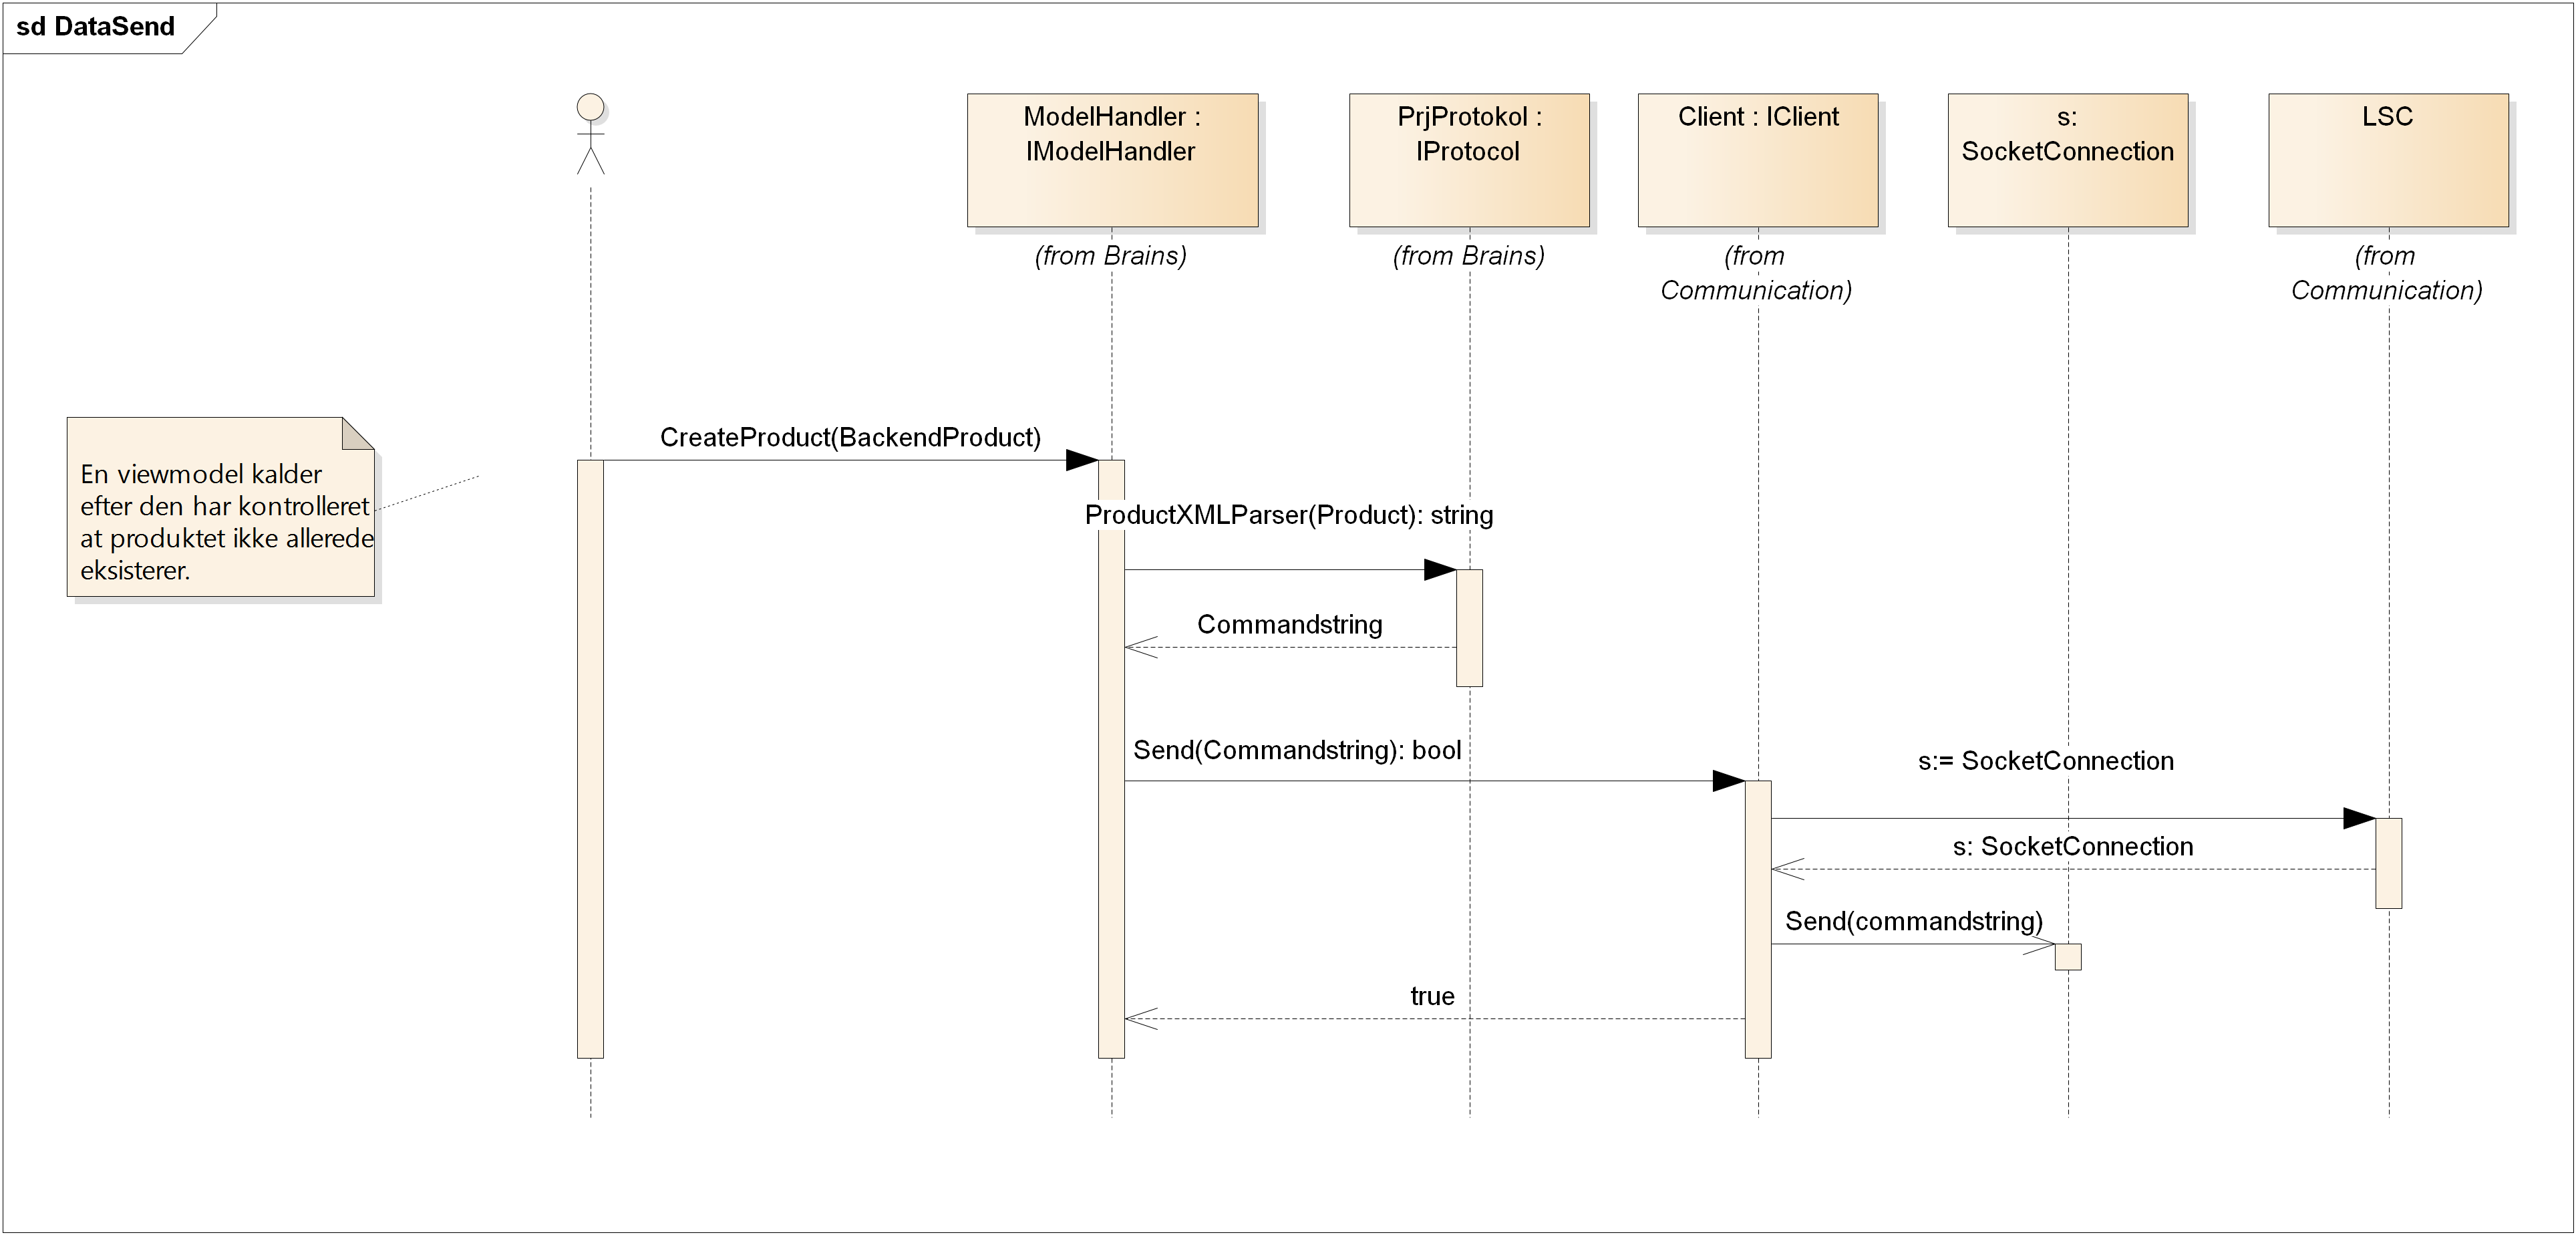
\includegraphics[width=1\textwidth]{Systemdesign/backend/Images/DataSend.png}
    \caption{Eksempel på hvordan CreateProduct bliver behandlet i systemet og sendt til Central Server}
    \label{fig:CreateSend}
\end{figure}

Derefter afsluttes der. Det betyder at når der eksempelvis oprettes et nyt produkt, bliver der ikke opdateret noget i systemet, der bliver udelukkende sendt data til serveren.\\


For at modtage data, subscriber MainWindowViewModel på nogle forskellige events, som eksempelvis OnProductCategoryDeleted, OnProductEdited mf. Dette gøres igennem klassen SocketEventHandlers [Ref], som også indeholder de eventhandlere der bliver kaldt, når et event raises på serveren.  Det er derfor disse eventhandlere som håndtere dataen, og lægger den nye data ind i datamodellerne – og det er først der, der bliver opdateret lokalt. På den måde vil der aldrig eksistere noget i databasen der ikke eksisterer i Administrationssystemet og vice versa. 
\begin{figure}[!h]
    \centering
    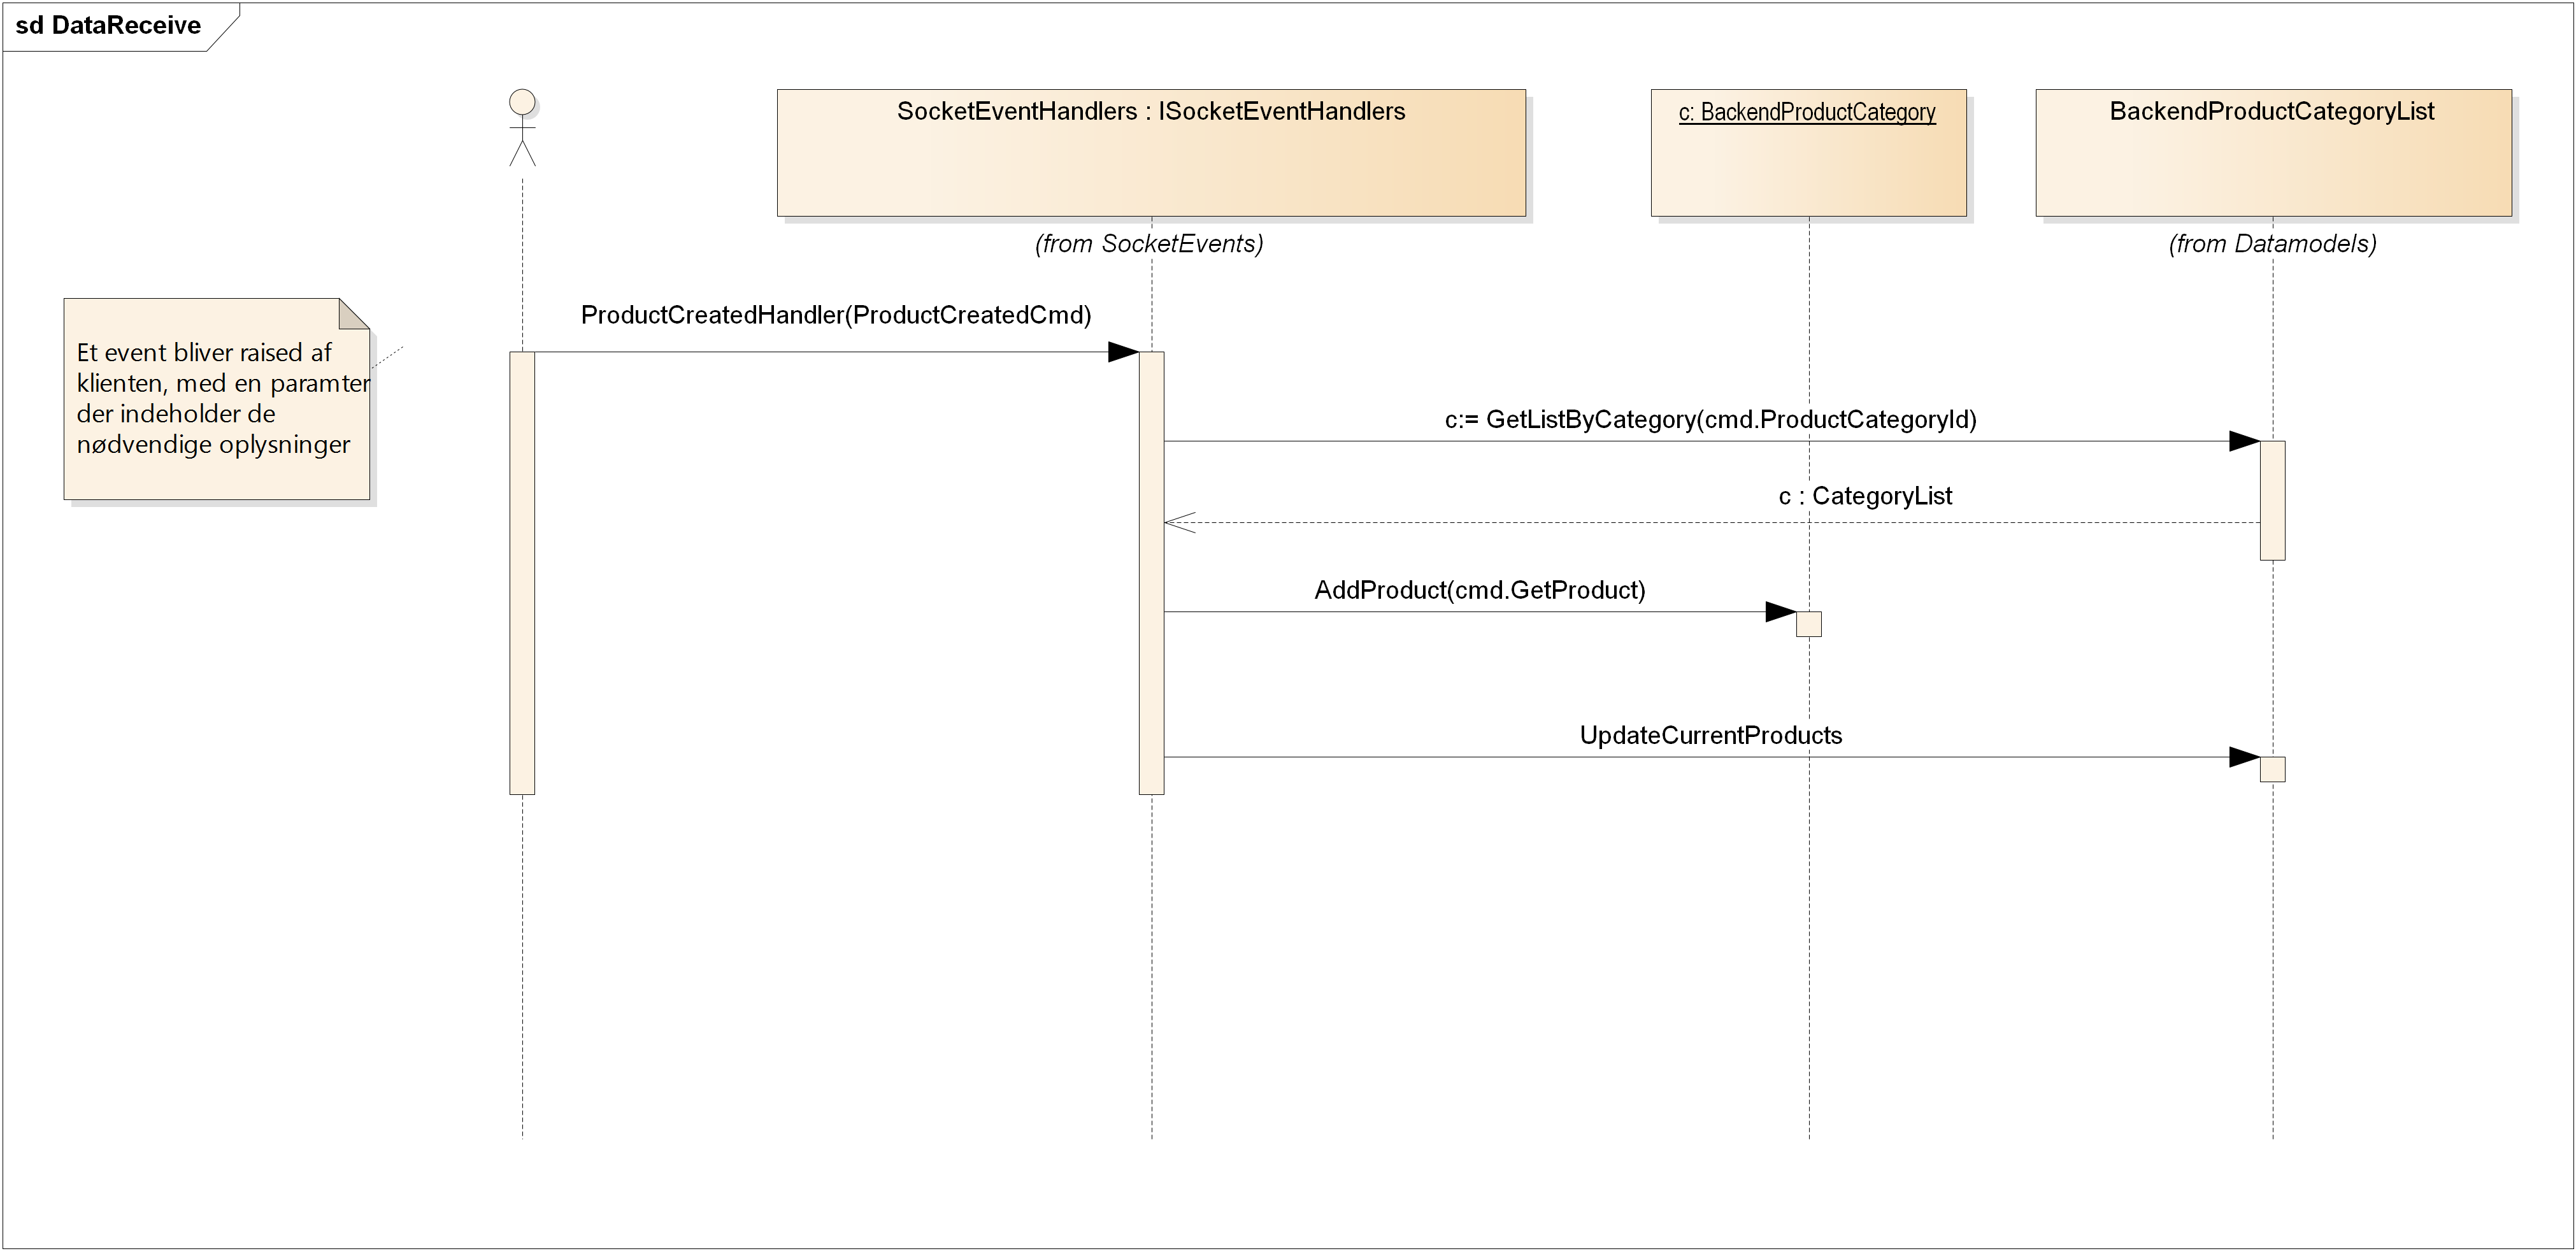
\includegraphics[width=1\textwidth]{Systemdesign/backend/Images/DataReceive.png}
    \caption{Eksempel på hvordan produktet igen bliver modtaget fra serveren, efter det er blevet oprettet.}
    \label{fig:DataReceive}
\end{figure}



\paragraph*{Kommunikation med Central Server}
Klienten i Administrationssystemet består af en socketconnection som er defineret i SharedLib[Ref]. Da denne skal bruges i både businesslogic, men også i MainWindowViewModel og der samtidig øn-skes at den samme benyttes hver gang, bruges Singleton[Reference] for denne forbindelse. \\
Til at sende data benyttes en ModelHandler [Ref], som hver i sær har en metode til de forskellige handlinger. Eksempelvis EditProduct, DeleteProduct mf. Disse metoder arbejder alle sammen på samme måde:
\begin{enumerate}
\item Opret en XML-kommandostring vha. protokollen [\textbf{REFERENCE TIL PROTOKOLLEN}]
\item Send data til klienten
\end{enumerate}


\begin{figure}[!h]
    \centering
    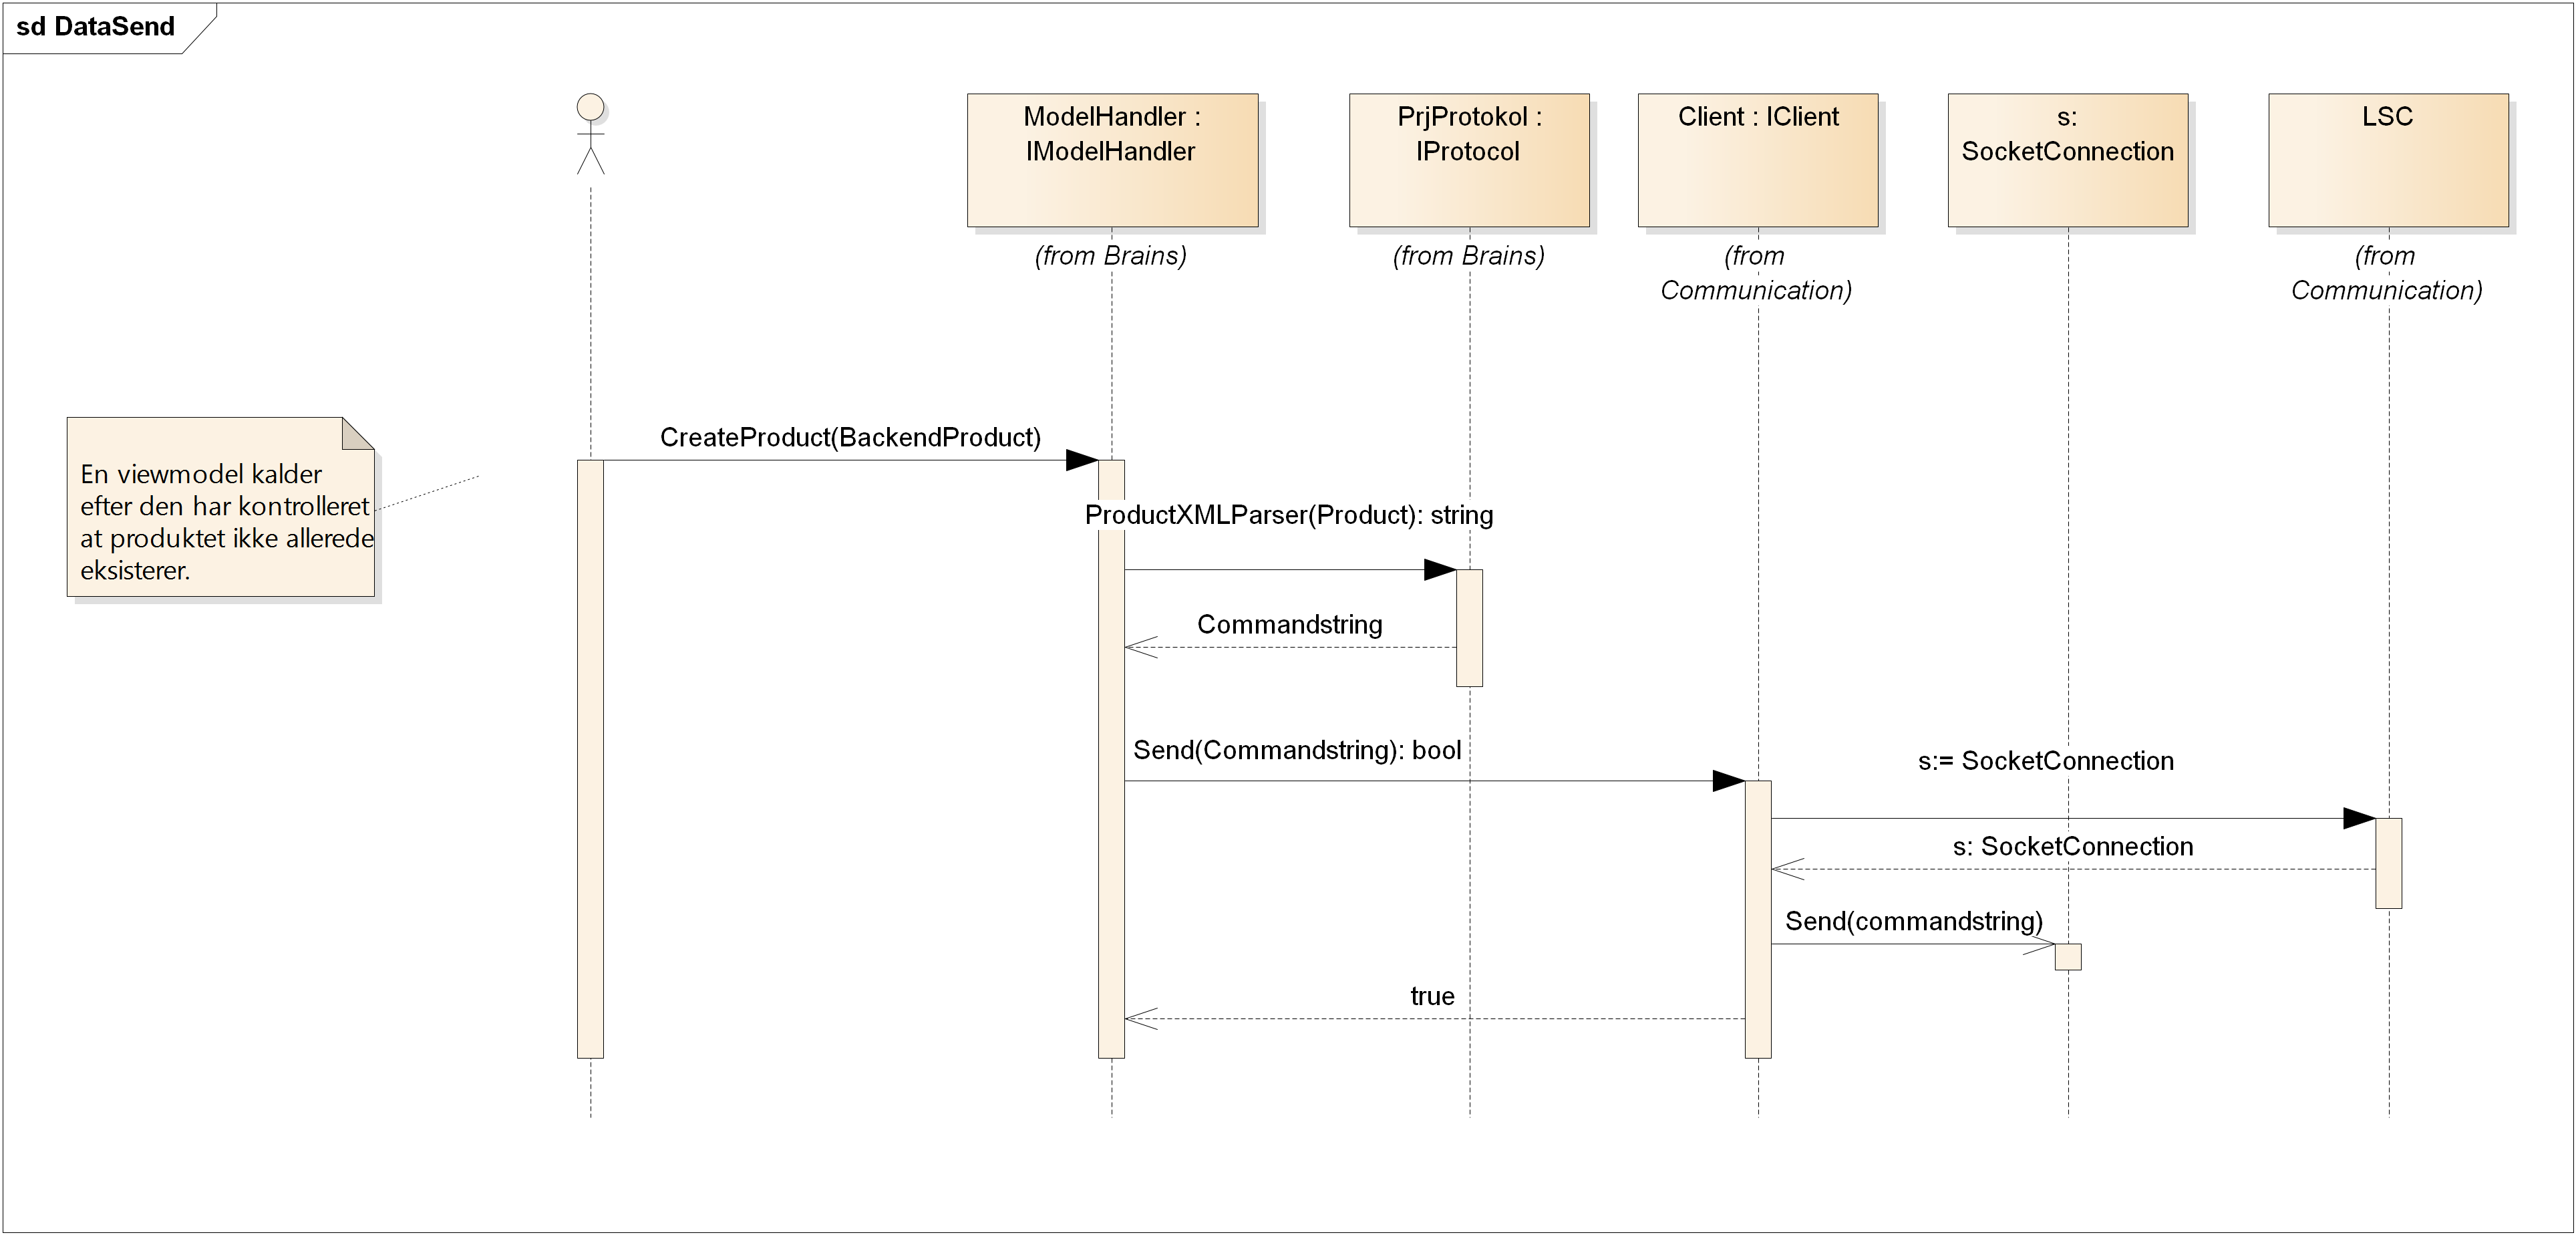
\includegraphics[width=1\textwidth]{Systemdesign/backend/Images/DataSend.png}
    \caption{Eksempel på hvordan CreateProduct bliver behandlet i systemet og sendt til Central Server}
    \label{fig:CreateSend}
\end{figure}

Derefter afsluttes der. Det betyder at når der eksempelvis oprettes et nyt produkt, bliver der ikke opdateret noget i systemet, der bliver udelukkende sendt data til serveren.\\


For at modtage data, subscriber MainWindowViewModel på nogle forskellige events, som eksempelvis OnProductCategoryDeleted, OnProductEdited mf. Dette gøres igennem klassen SocketEventHandlers [Ref], som også indeholder de eventhandlere der bliver kaldt, når et event raises på serveren.  Det er derfor disse eventhandlere som håndtere dataen, og lægger den nye data ind i datamodellerne – og det er først der, der bliver opdateret lokalt. På den måde vil der aldrig eksistere noget i databasen der ikke eksisterer i Administrationssystemet og vice versa. 
\begin{figure}[!h]
    \centering
    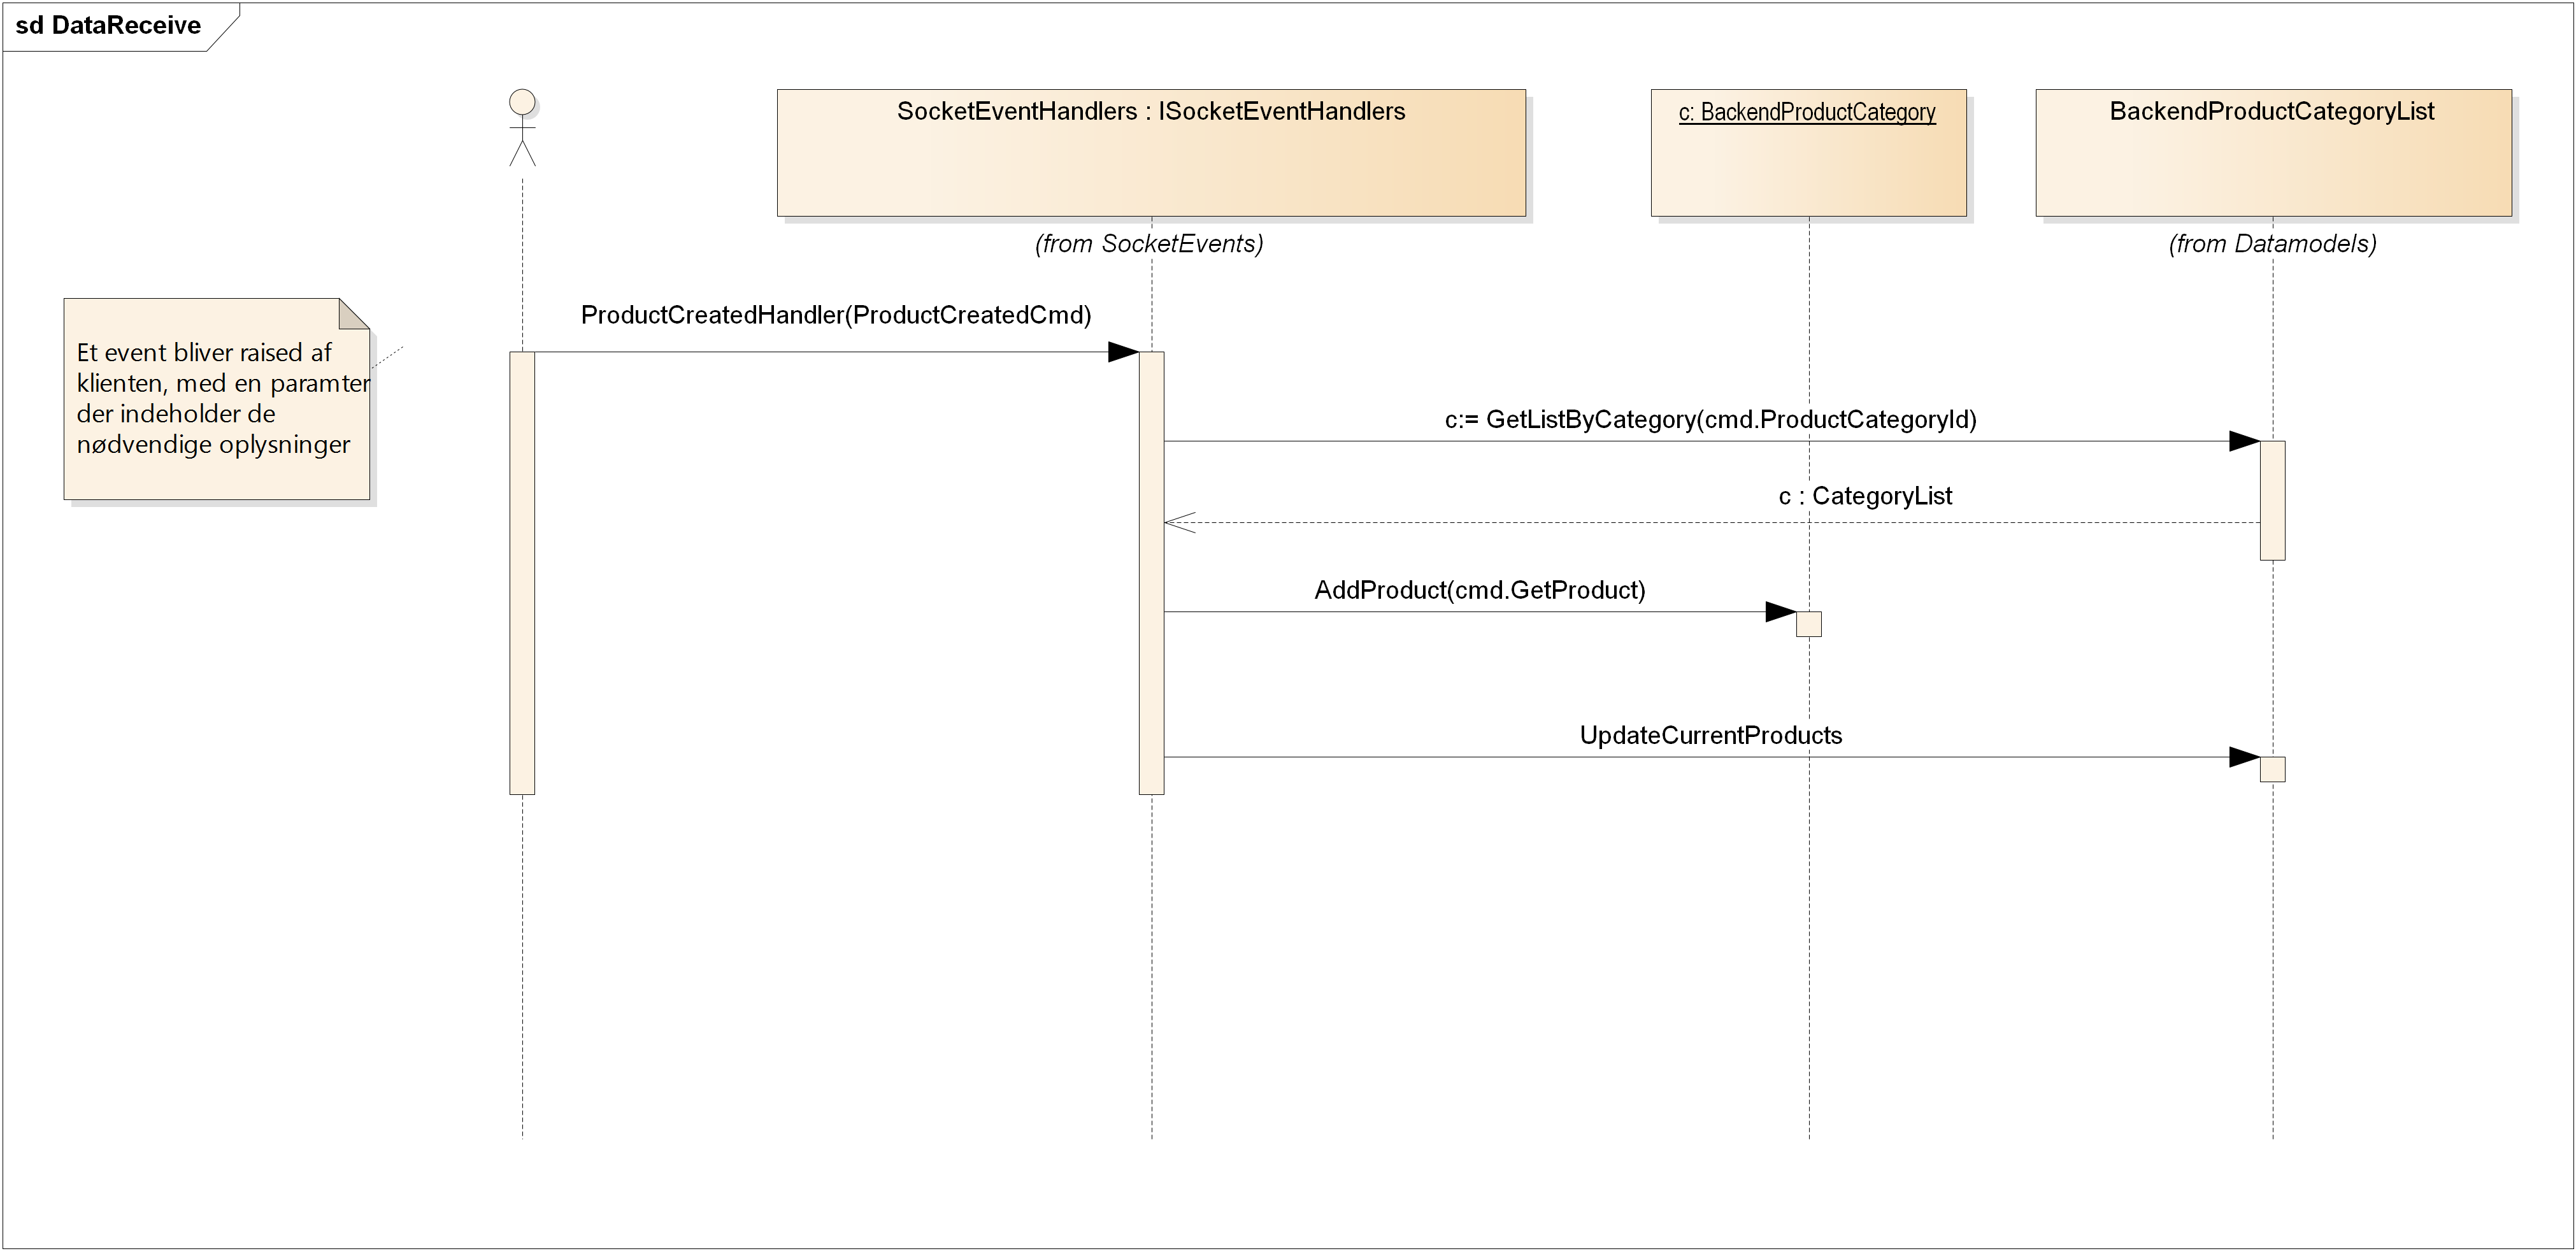
\includegraphics[width=1\textwidth]{Systemdesign/backend/Images/DataReceive.png}
    \caption{Eksempel på hvordan produktet igen bliver modtaget fra serveren, efter det er blevet oprettet.}
    \label{fig:DataReceive}
\end{figure}



\paragraph*{Kommunikation med Central Server}
Klienten i Administrationssystemet består af en socketconnection som er defineret i SharedLib[Ref]. Da denne skal bruges i både businesslogic, men også i MainWindowViewModel og der samtidig øn-skes at den samme benyttes hver gang, bruges Singleton[Reference] for denne forbindelse. \\
Til at sende data benyttes en ModelHandler [Ref], som hver i sær har en metode til de forskellige handlinger. Eksempelvis EditProduct, DeleteProduct mf. Disse metoder arbejder alle sammen på samme måde:
\begin{enumerate}
\item Opret en XML-kommandostring vha. protokollen [\textbf{REFERENCE TIL PROTOKOLLEN}]
\item Send data til klienten
\end{enumerate}


\begin{figure}[!h]
    \centering
    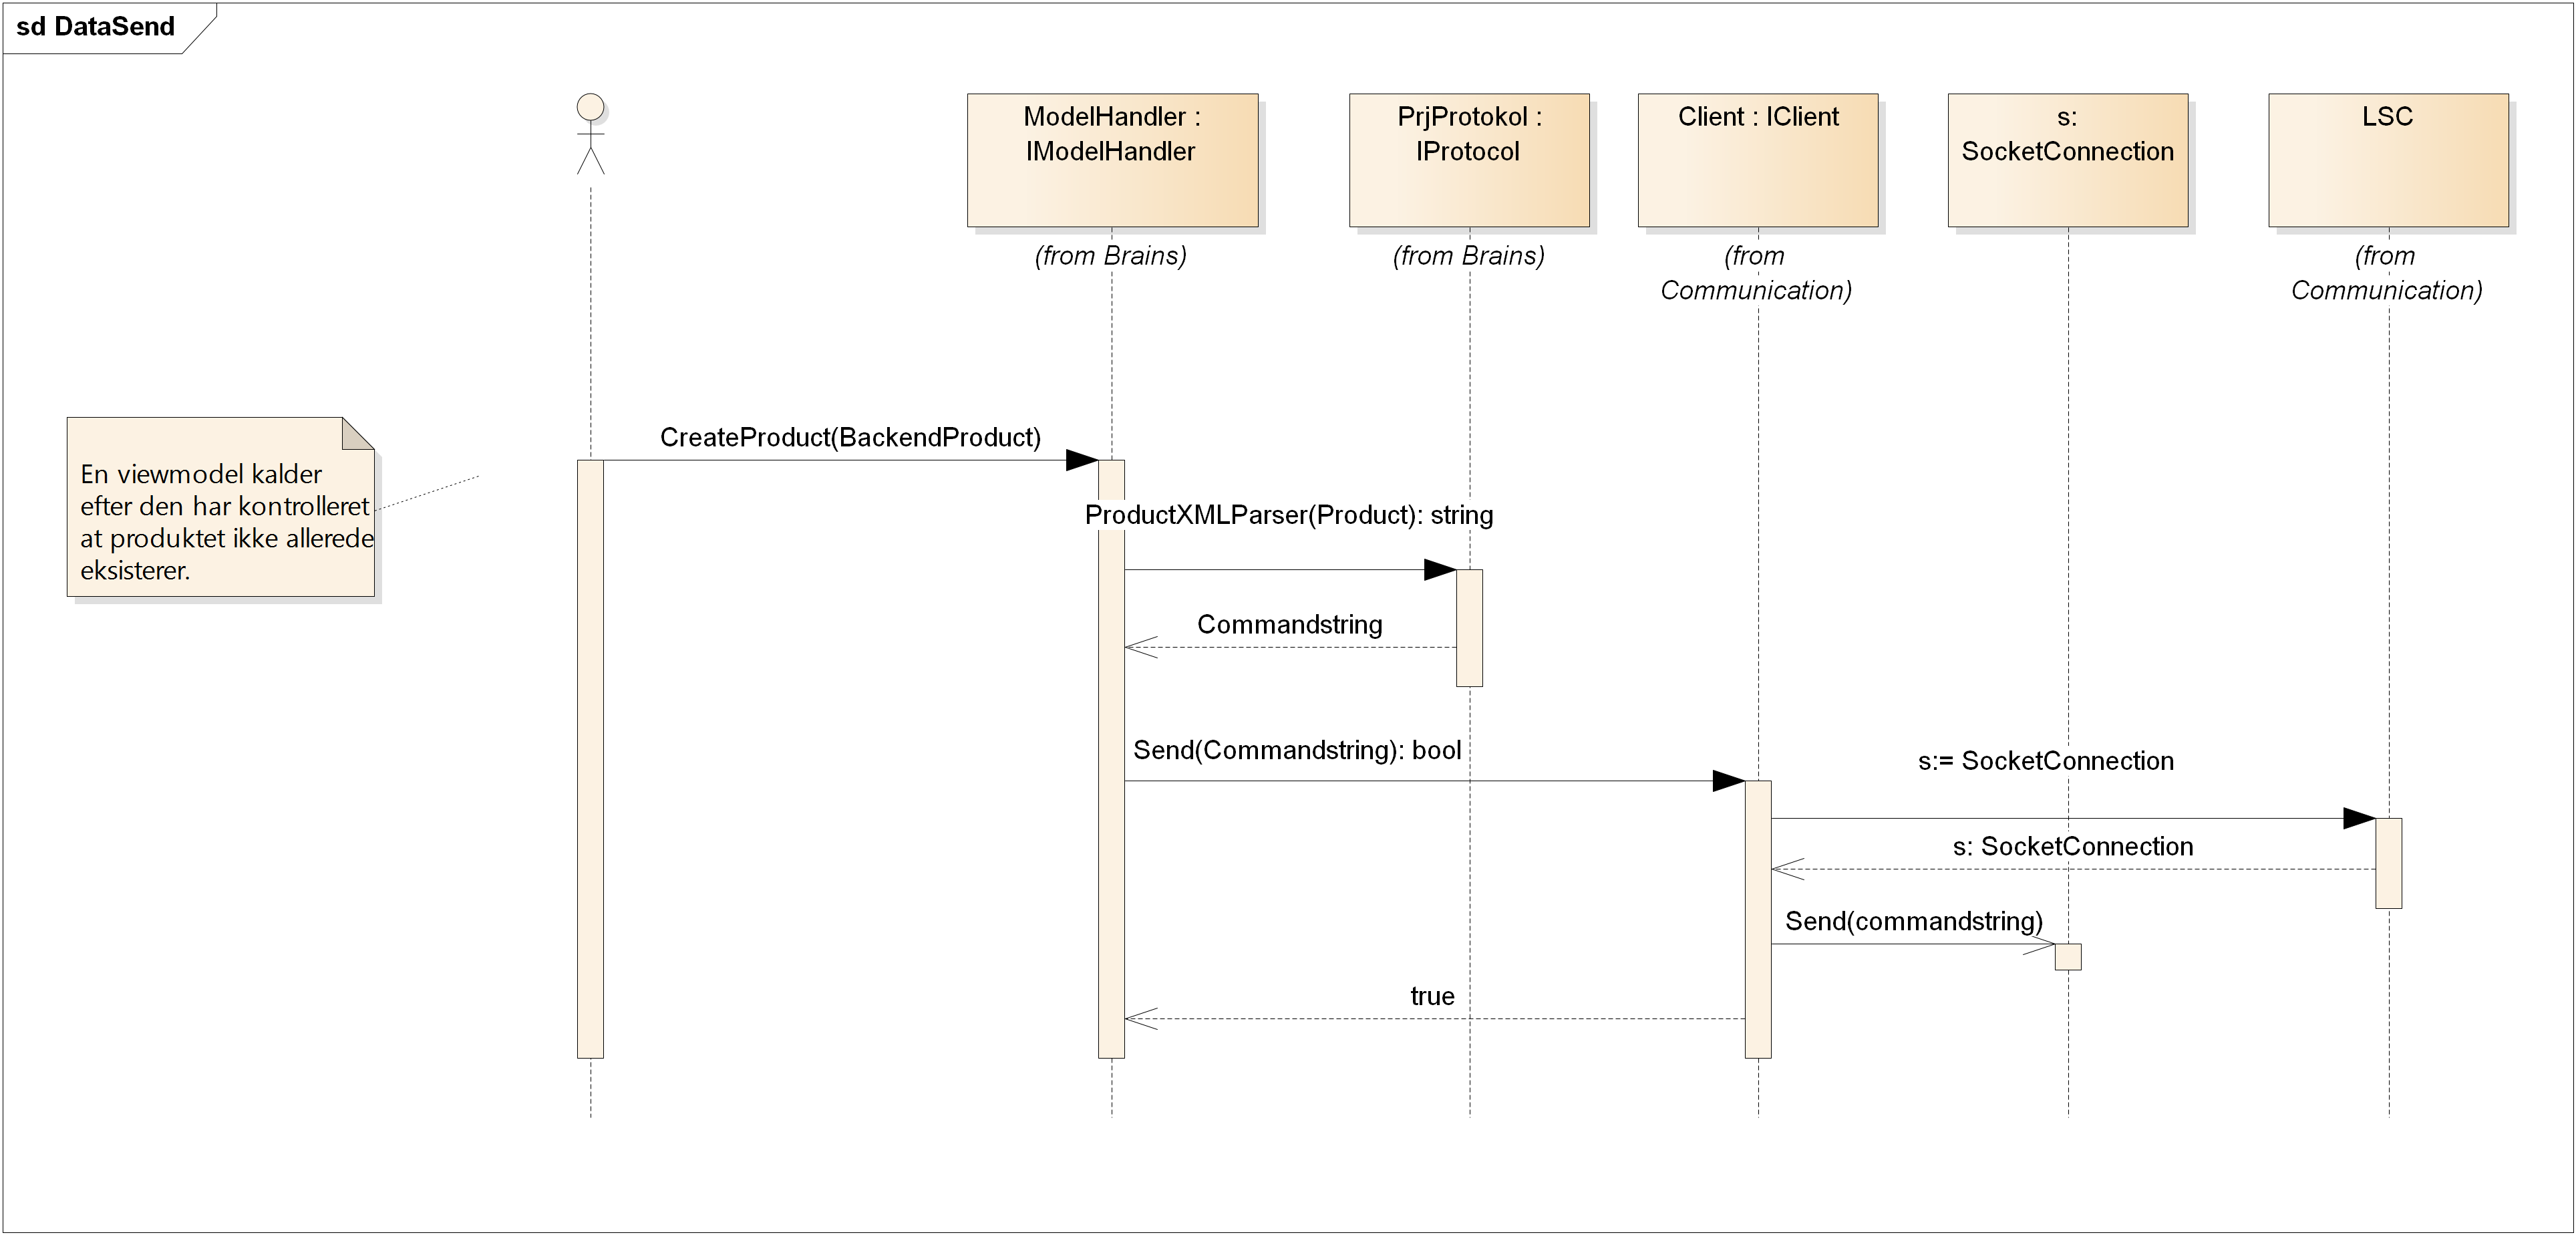
\includegraphics[width=1\textwidth]{Systemdesign/backend/Images/DataSend.png}
    \caption{Eksempel på hvordan CreateProduct bliver behandlet i systemet og sendt til Central Server}
    \label{fig:CreateSend}
\end{figure}

Derefter afsluttes der. Det betyder at når der eksempelvis oprettes et nyt produkt, bliver der ikke opdateret noget i systemet, der bliver udelukkende sendt data til serveren.\\


For at modtage data, subscriber MainWindowViewModel på nogle forskellige events, som eksempelvis OnProductCategoryDeleted, OnProductEdited mf. Dette gøres igennem klassen SocketEventHandlers [Ref], som også indeholder de eventhandlere der bliver kaldt, når et event raises på serveren.  Det er derfor disse eventhandlere som håndtere dataen, og lægger den nye data ind i datamodellerne – og det er først der, der bliver opdateret lokalt. På den måde vil der aldrig eksistere noget i databasen der ikke eksisterer i Administrationssystemet og vice versa. 
\begin{figure}[!h]
    \centering
    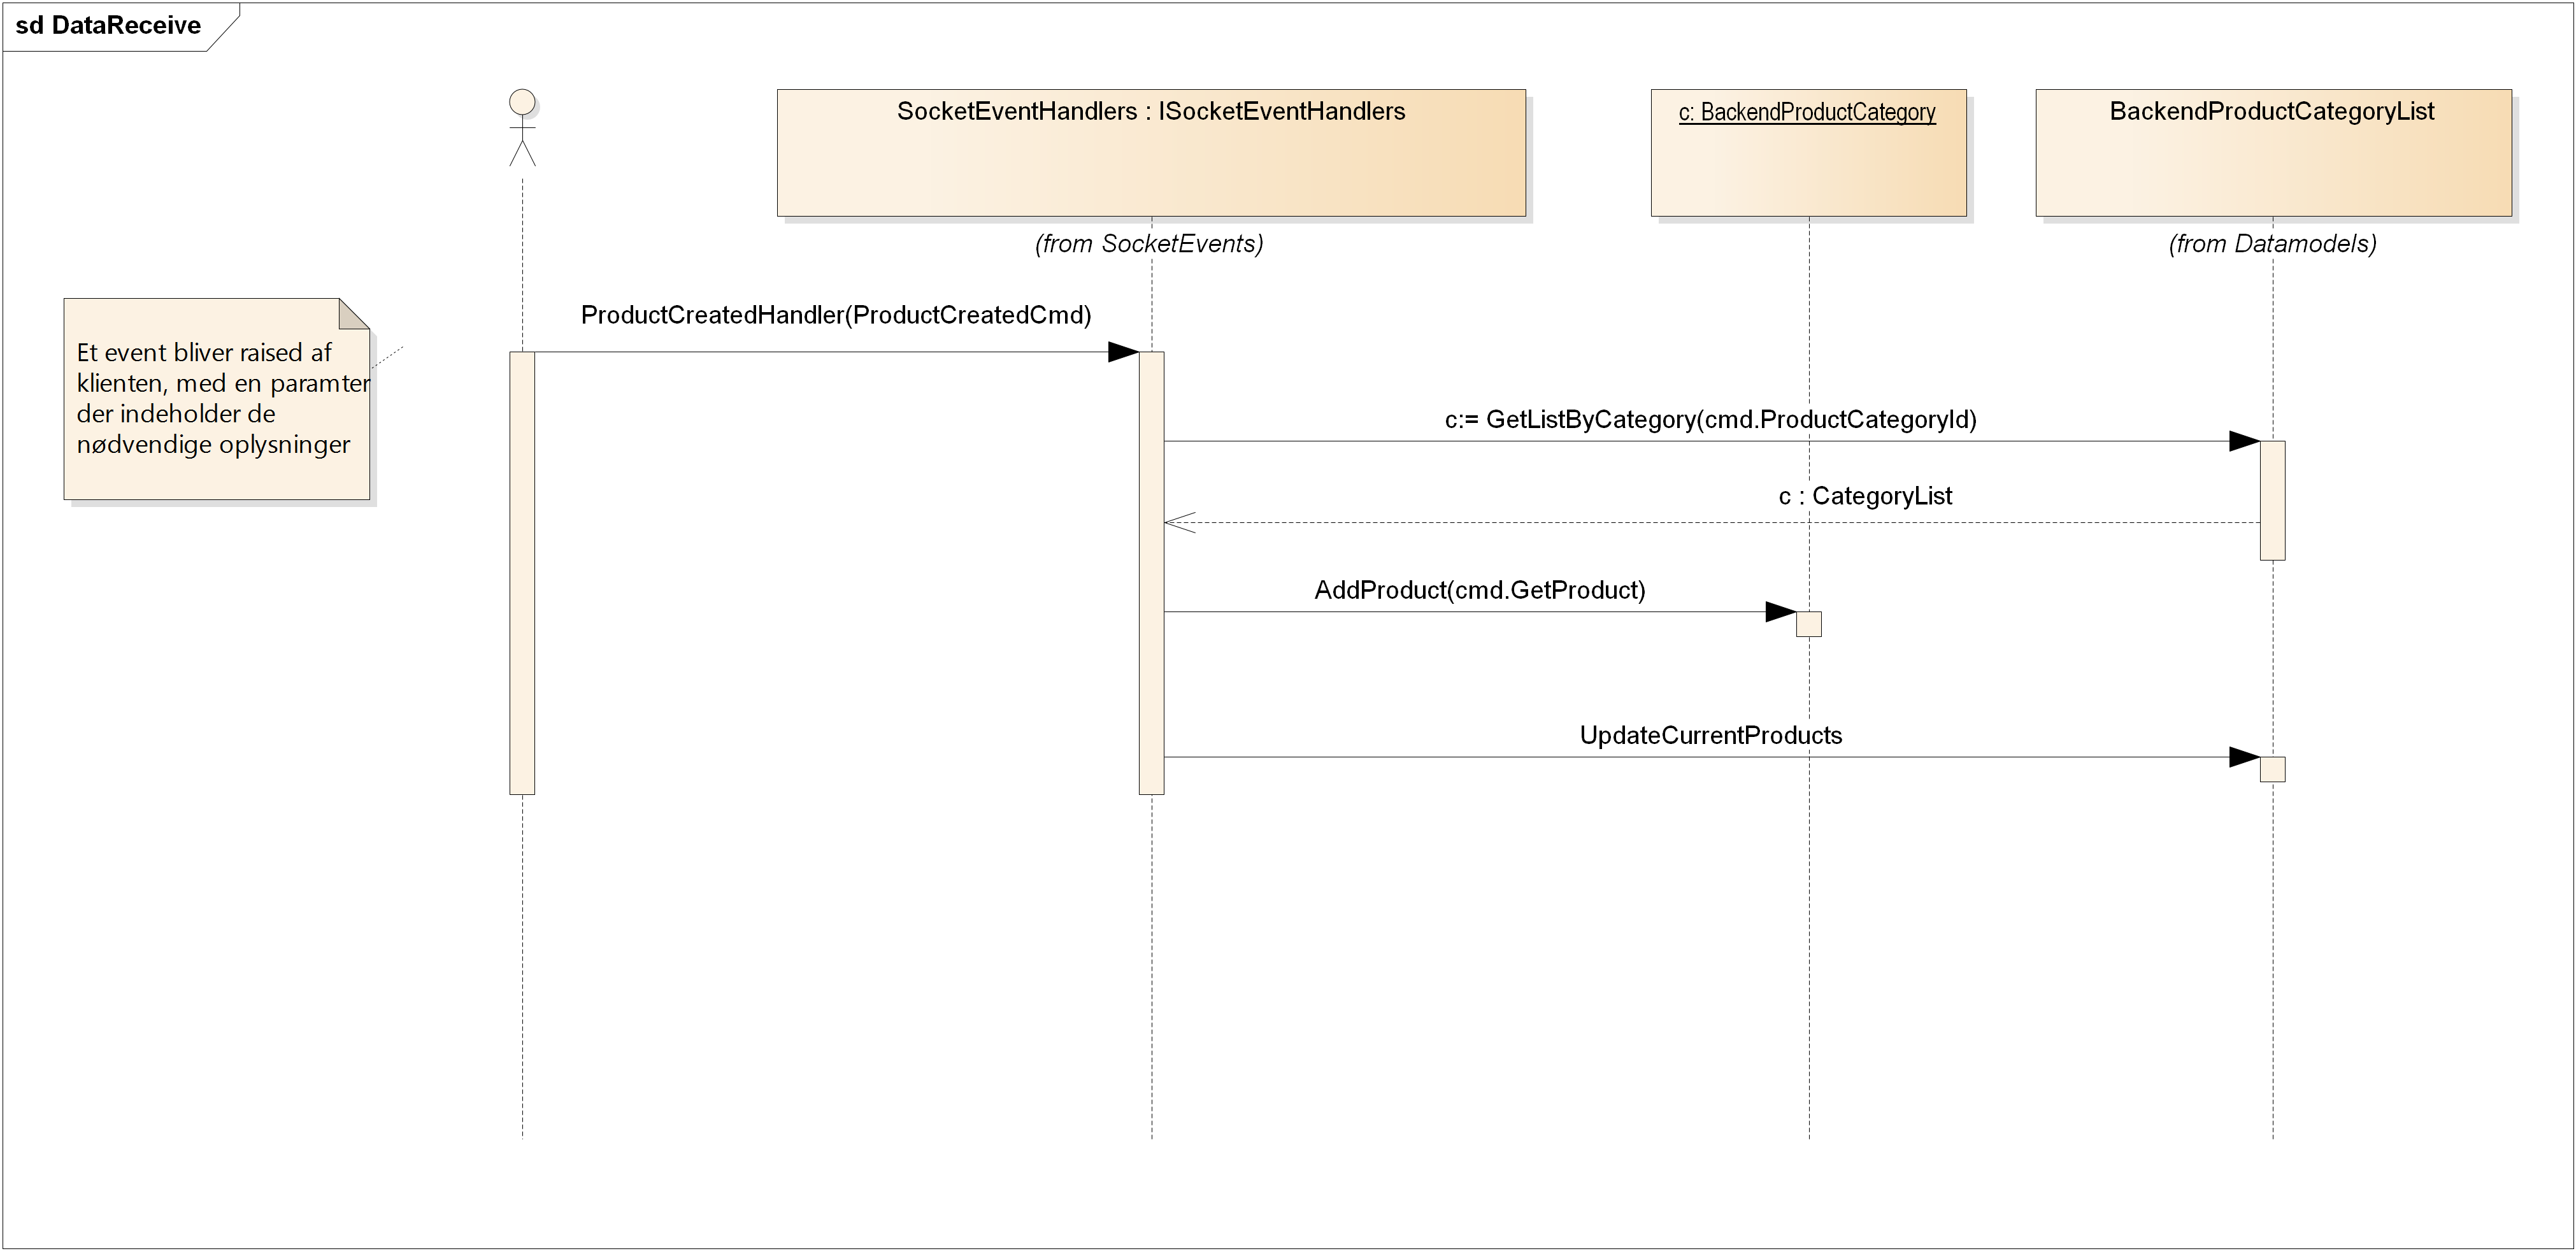
\includegraphics[width=1\textwidth]{Systemdesign/backend/Images/DataReceive.png}
    \caption{Eksempel på hvordan produktet igen bliver modtaget fra serveren, efter det er blevet oprettet.}
    \label{fig:DataReceive}
\end{figure}



\subsubsection{Kommunikation med Central Server}
Klienten i Administrationssystemet består af en socketconnection som er defineret i SharedLib[Ref]. Da denne skal bruges i både businesslogic, men også i MainWindowViewModel og der samtidig øn-skes at den samme benyttes hver gang, bruges Singleton[Reference] for denne forbindelse. \\
Til at sende data benyttes en ModelHandler [Ref], som hver i sær har en metode til de forskellige handlinger. Eksempelvis EditProduct, DeleteProduct mf. Disse metoder arbejder alle sammen på samme måde:
\begin{enumerate}
\item Opret en XML-kommandostring vha. protokollen\footnote{Nærmere beskrivet under SharedLib, afsnit \ref{SHAREDLIB}, side \pageref{SHAREDLIB}}
\item Send data til klienten
\end{enumerate}


\begin{figure}[!h]
    \centering
    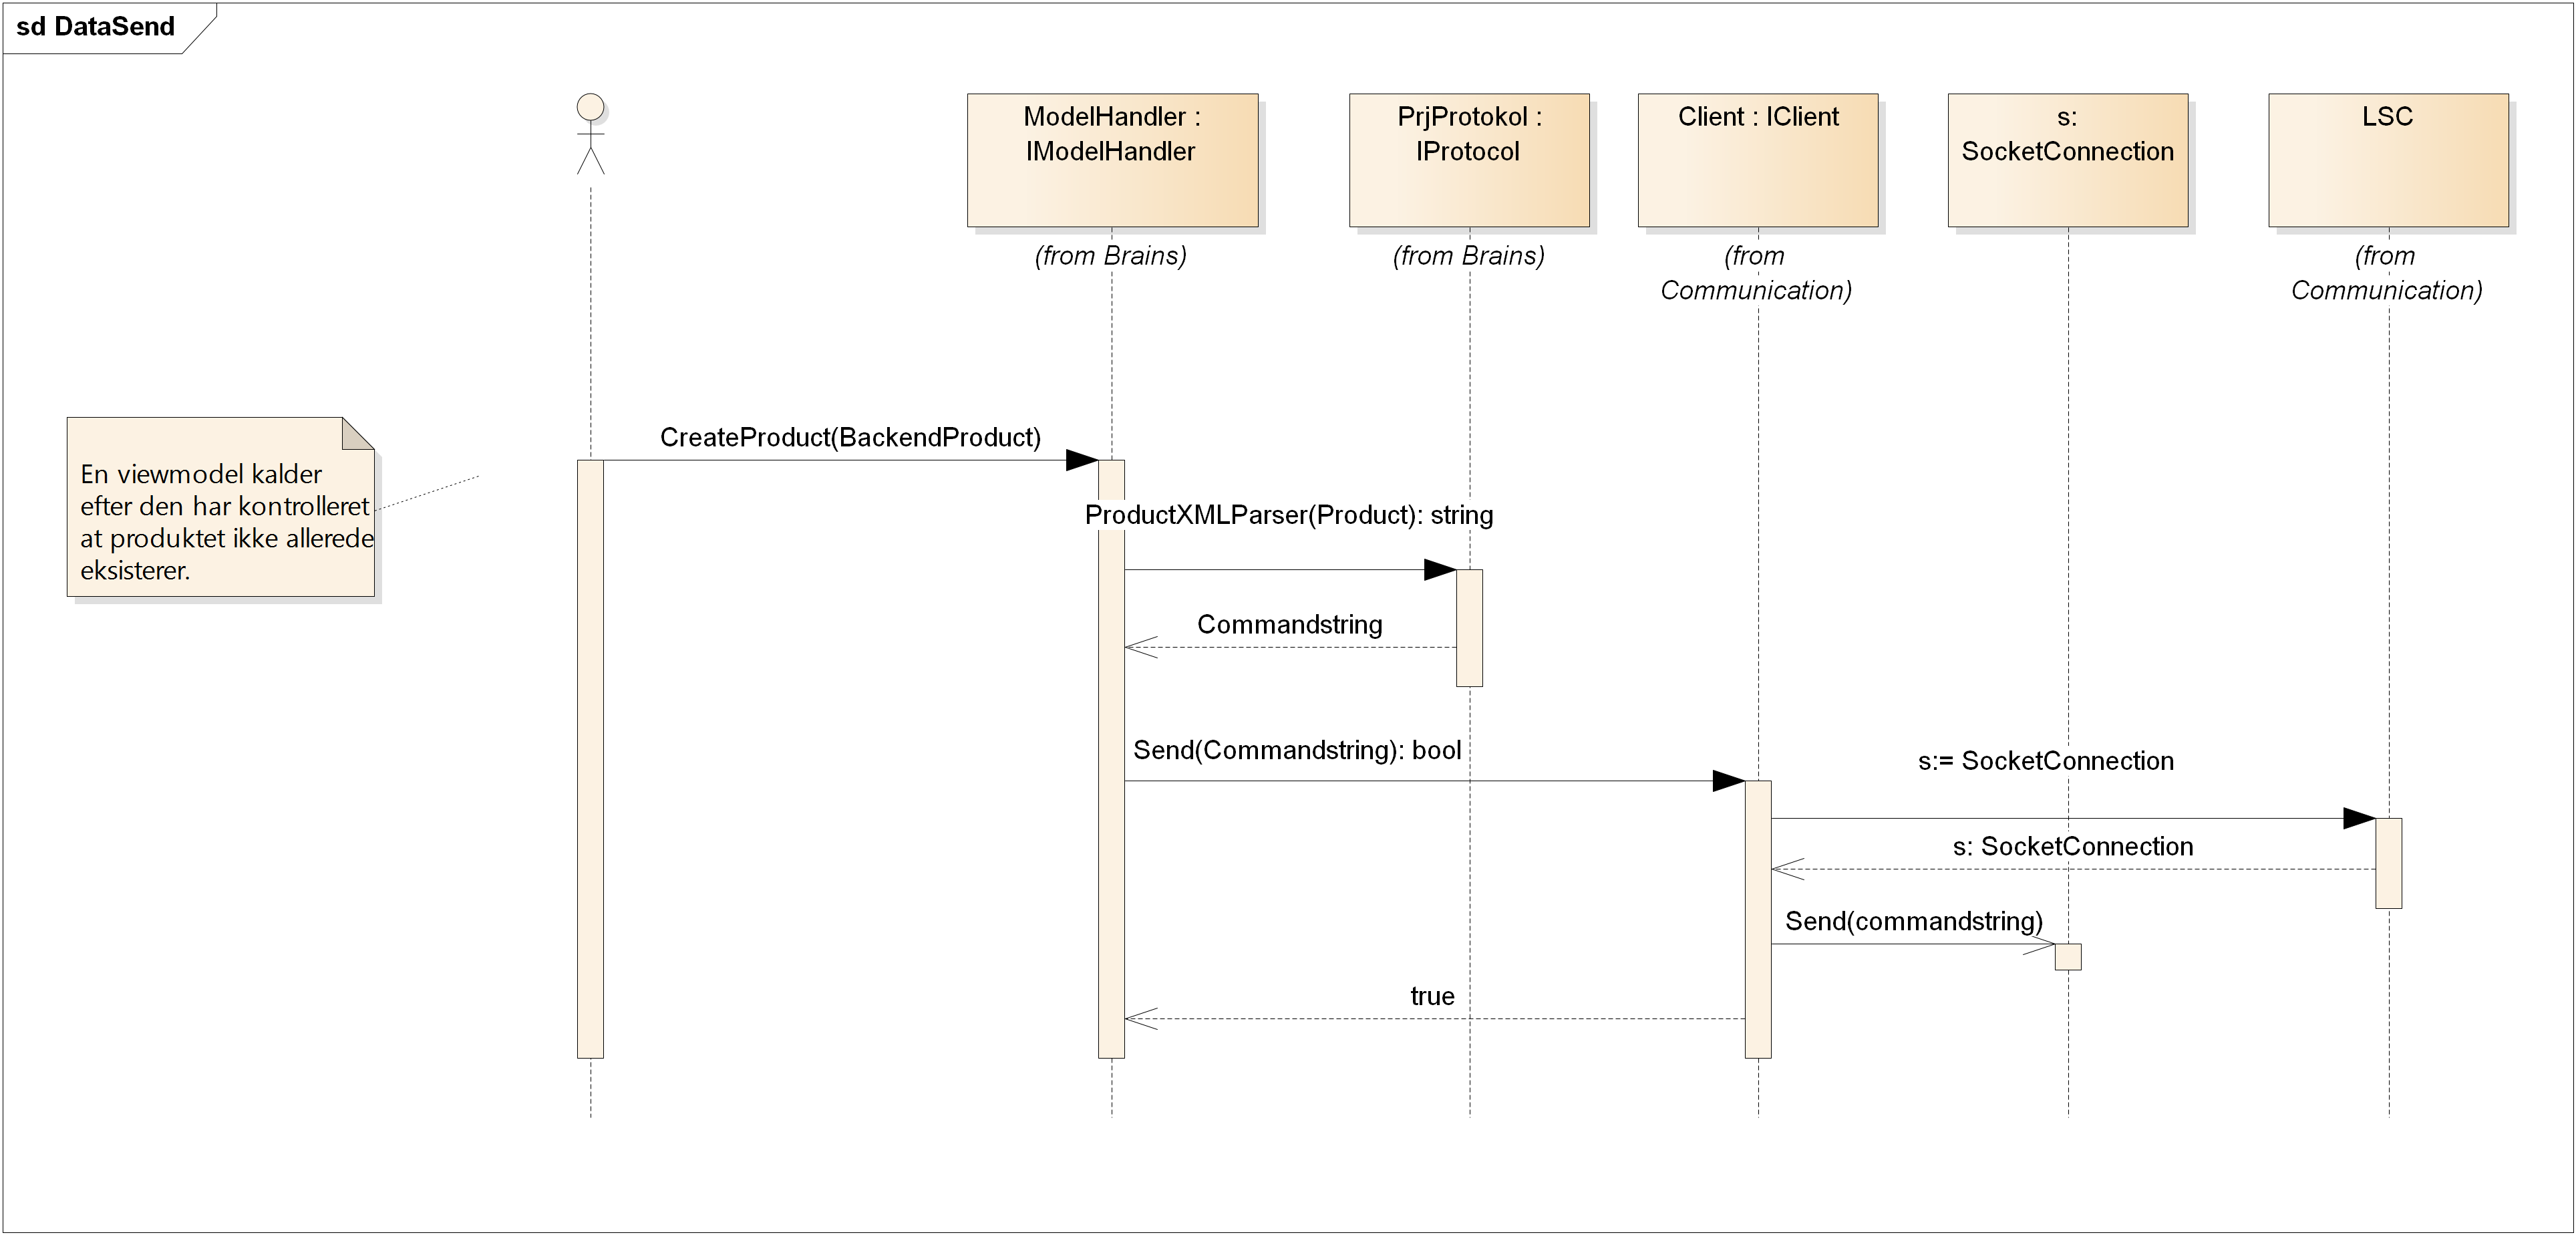
\includegraphics[width=1\textwidth]{Systemdesign/backend/Images/DataSend.png}
    \caption{Eksempel på hvordan CreateProduct bliver behandlet i systemet og sendt til Central Server}
    \label{fig:CreateSend}
\end{figure}

På figur \ref{fig:CreateSend} ses det hvordan en viewmodel kunne kalde CreateProduct i ModelHandler\footnote{Nærmere beskrevet under klassebeskrivelser, afsnit \ref{Modelhandler_Beskrivelse} side \pageref{Modelhandler_Beskrivelse}}, som får lavet en XML-streng \gls{CS} kan forstå. Derefter bliver denne data sendt ud igennem en socket forbindelse.
Derefter afsluttes der. Det betyder at når der eksempelvis oprettes et nyt produkt, bliver der ikke opdateret noget i systemet, der bliver udelukkende sendt data til \gls{CS}.\\\\


For at modtage data, subscriber MainWindowViewModel på nogle forskellige events, som eksempelvis OnProductCategoryDeleted, OnProductEdited mf. Dette gøres igennem klassen SocketEventHandlers\footnote{Nærmere beskrevet under klassebeskrivelser, afsnit \ref{SocketEventHandlerBeskrivelse} side \pageref{SocketEventHandlerBeskrivelse}}, som også indeholder de eventhandlere der bliver kaldt, når et event raises på serveren.  Det er derfor disse eventhandlere som håndtere dataen, og lægger den nye data ind i datamodellerne – og det er først der, der bliver opdateret lokalt. På den måde vil der aldrig eksistere noget i databasen der ikke eksisterer i Administrationssystemet og vice versa. 
\begin{figure}[!h]
    \centering
    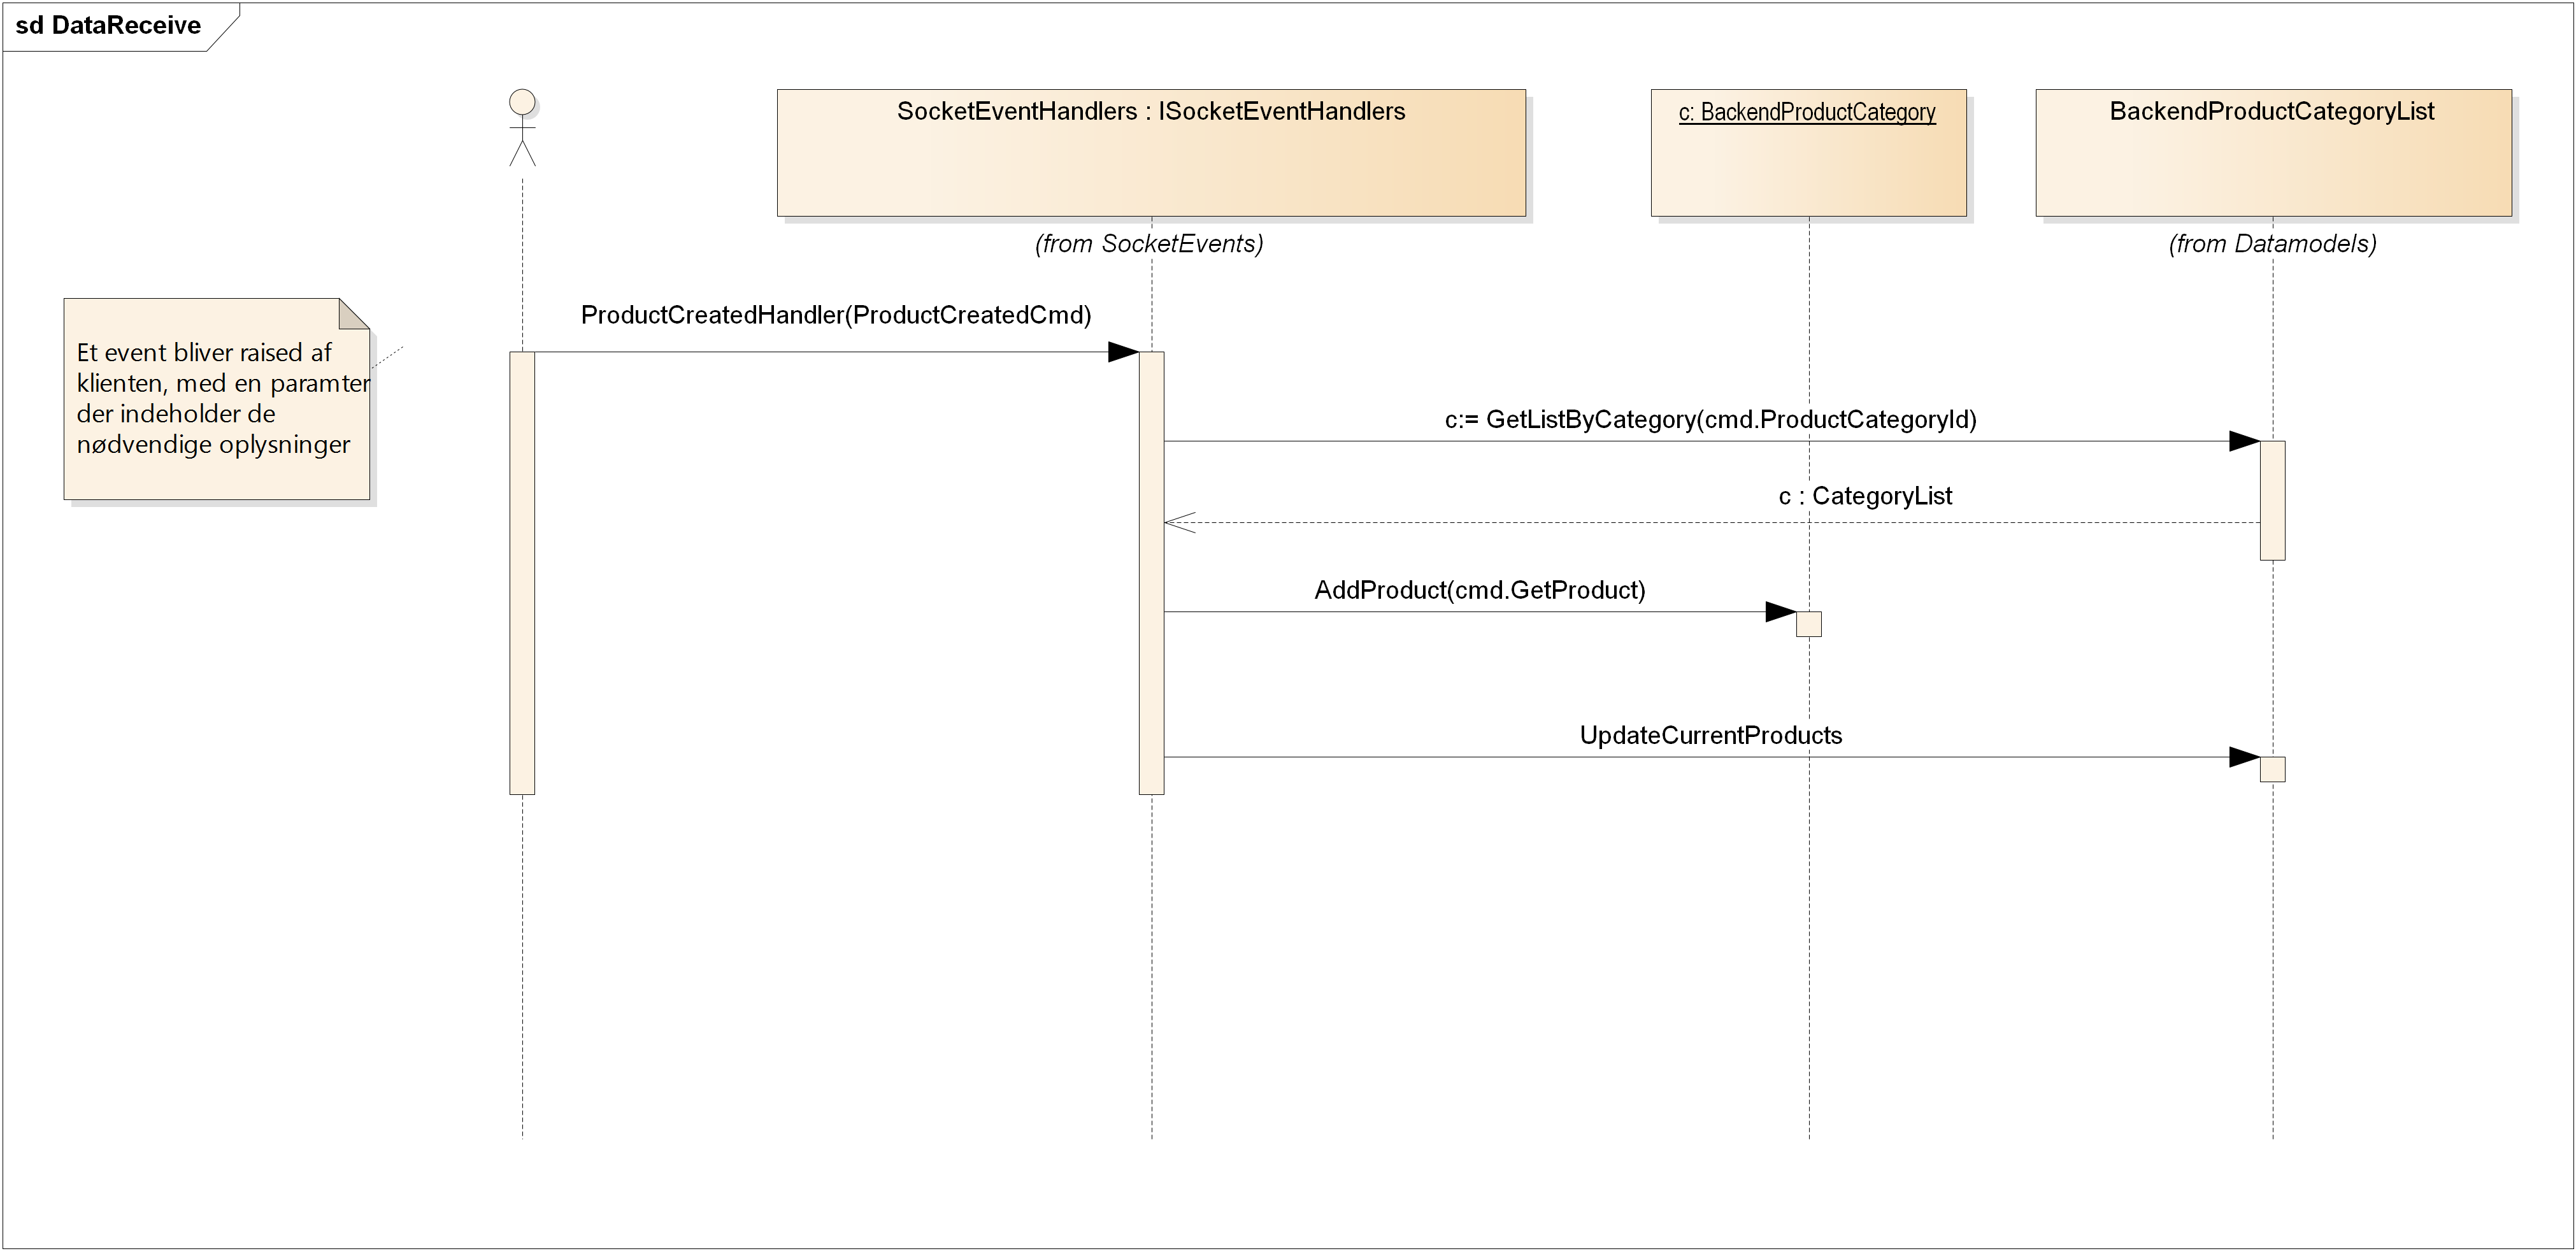
\includegraphics[width=1\textwidth]{Systemdesign/backend/Images/DataReceive.png}
    \caption{Eksempel på hvordan produktet igen bliver modtaget fra serveren, efter det er blevet oprettet.}
    \label{fig:DataReceive}
\end{figure}    

På figur \ref{fig:DataReceive} ses det hvordan et event bliver raised, og den rigtige eventhandler bliver kaldt, på baggrund af de subscribtions der blev lavet i MainViewViewModel. Først efter at denne har tilføjet produktet til den interne produktliste, er produktet synlig i programmet. Det er derfor \gls{CS} der bestemmer hvornår et produkt blive tilføjet, fjernet eller redigeret.\\
\\
Dette er gjort således at der ikke, ved en fejl, kunne opstå problemer med at et produkt i \gls{AS} ikke stemmer overens - eller overhovedet eksisteret - i \gls{CS}. Desuden tillader dette også at flere noder kan lytte på disse events, så hvis en anden node eksempelvis tilføjer et produkt, så bliver listen i alle andre noder også opdateret. Det er besluttet at der skal subscribes på events enkeltvis, således det er muligt at have noder der kun er interesseret i en del af dataen, kun at få denne data. 
Der kan derfor sikres at \textit{alle} med forbindelse til \gls{CS} er fuldt opdateret på de ting de subscriber på.

